%! TEX root = main.tex

\graphicspath{{00_Images/07_chapter/}}

\chapter{Loudspeaker Dynamics and Resonance}
\label{ch:dynamics}

The complete mechanical section of the loudspeaker, established in the previous chapters, can now be analyzed as a resonant system driven by an electrical source.
The interplay between the suspension compliance and the diaphragm mass produces a mechanical resonance at the fundamental frequency \(f_s\); the quality factor of this resonance governs the shape of the impedance peak, the diaphragm velocity, displacement, and acceleration across the audio band.
This chapter derives the resonance and quality-factor expressions from the equivalent circuit, then traces the frequency-dependent behavior of all three kinematic quantities.

\section{RLC Resonant System}
\label{sc:71}

The mechanical section of the loudspeaker is a second-order resonant system.
Under the admittance analogy, the diaphragm mass \(M_{MS}\), suspension compliance \(C_{MS}\), and total mechanical resistance \(R_M = R_{ME} + R_{MS} + R_{MR}\) form a parallel RLC network in which velocity \(u_C\) plays the role of voltage and force \(F_C\) plays the role of current.
Under the impedance analogy, the same three elements form a series RLC network in which velocity is the shared current and the driving force is the loop voltage.
Both representations are physically equivalent and produce identical predictions once all quantities are referred to the same domain.

\begin{figure}[!htb]
    \centering
    \subfloat[Parallel RLC (admittance analogy)]{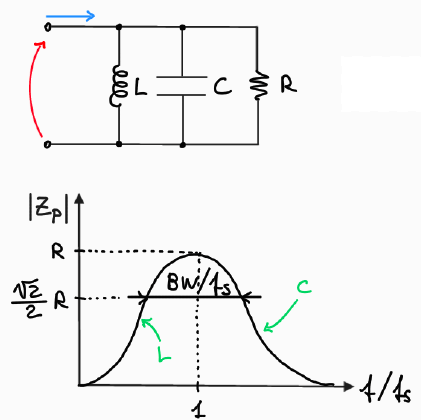
\includegraphics[width=0.50\linewidth]{parallel_RLC_with_Q.png}}
    \\
    \subfloat[Series RLC (impedance analogy)]{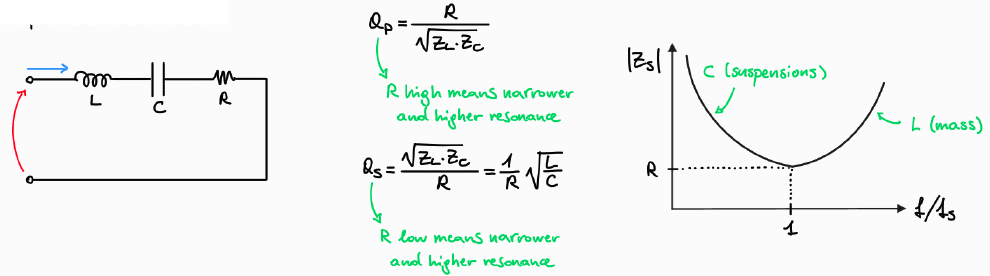
\includegraphics[width=0.85\linewidth]{parallel_to_series_RLC.png}}
    \caption{The mechanical section of the loudspeaker modeled as a parallel RLC resonator (admittance analogy, left) and as a series RLC resonator (impedance analogy, right). The resonance frequency \(f_s\) and the quality factor \(Q\) are identical in both representations; only the circuit topology differs}
\end{figure}

\subsection{Resonance Frequency}
\label{ssc:711}

The resonance condition is reached when the inductive and capacitive reactances cancel.
For the parallel network (admittance analogy), this occurs at:
\[
\omega_s L_{ES} = \frac{1}{\omega_s C_{ED}}
\qquad\Longrightarrow\qquad
\omega_s = \frac{1}{\sqrt{L_{ES} C_{ED}}}
\]
Substituting the electrical equivalents \(L_{ES} = (Bl)^2 C_{MS}\) and \(C_{ED} = M_{MS}/(Bl)^2\):
\[
\omega_s = \frac{1}{\sqrt{(Bl)^2 C_{MS} \cdot M_{MS}/(Bl)^2}} = \frac{1}{\sqrt{M_{MS} C_{MS}}}
\]
The \(Bl\) factor cancels exactly, confirming that the resonance frequency is a purely mechanical parameter, independent of the electromagnetic coupling:
\begin{equation}
    f_s = \frac{1}{2\pi\sqrt{M_{MS} C_{MS}}}
    \label{eq:resonanceFrequency}
\end{equation}
At \(f = f_s\), the impedance of the parallel RLC reaches its maximum value \(R_{ES}\), the circuit behaves as a pure resistance, and the diaphragm velocity peaks at its maximum amplitude.
The bandwidth of the resonance peak, measured between the two frequencies \(f_H\) and \(f_L\) at which the impedance magnitude falls to \(1/\sqrt{2}\) of its maximum, is:
\[
Q = \frac{f_s}{f_H - f_L}
\]

\begin{figure}[!htb]
    \centering
    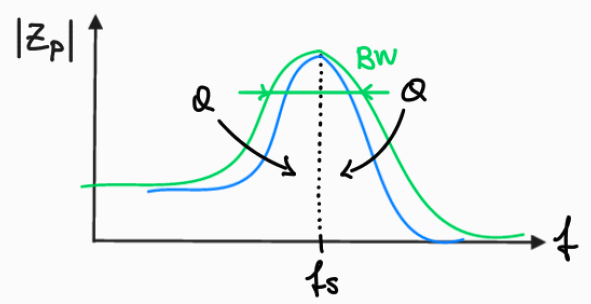
\includegraphics[width=0.50\linewidth]{Q_Factor_Graph.png}
    \caption{Influence of the quality factor \(Q\) on the magnitude response \(|Z_P(f)|\) of the parallel RLC. A higher \(Q\) produces a sharper resonance peak and a narrower bandwidth \(f_H - f_L\)}
\end{figure}

For the parallel RLC with resistance \(R\), inductance \(L\), and capacitance \(C\), the normalized impedance expression is:
\[
Z_P = R \frac{j\dfrac{1}{Q}\dfrac{f}{f_s}}{1 - \left(\dfrac{f}{f_s}\right)^2 + j\dfrac{1}{Q}\dfrac{f}{f_s}}
\]
where \(Q = R\sqrt{C/L}\).

\paragraph{Multiple RLC contributions} When the radiation resistance \(R_{MR}\) and the referred electrical resistance \(R_{ME}\) both appear alongside the suspension resistance \(R_{MS}\), the total mechanical resistance is their sum \(R_M = R_{ME} + R_{MS} + R_{MR}\).
Each contributes an independent quality factor, and the effective \(Q\) is controlled by the smallest individual contribution, in direct analogy with the parallel combination of resistors.

\begin{figure}[!htb]
    \centering
    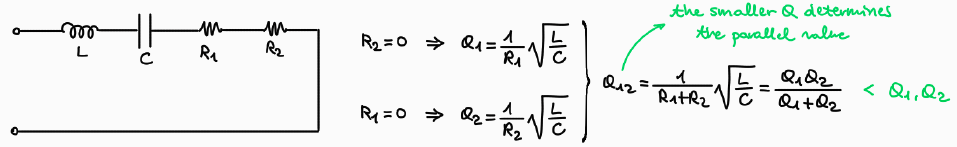
\includegraphics[width=0.85\linewidth]{multi_RLC_hint.png}
    \caption{Multiple RLC contributions to the mechanical branch. Each resistance defines its own quality factor; the effective parallel \(Q\) is dominated by the branch with the lowest \(Q\), i.e., the highest damping contribution}
\end{figure}

\section{Q-Factor Combination}
\label{sc:72}

The total damping of the loudspeaker system is quantified by the total quality factor \(Q_{TS}\), which collects both the mechanical losses in the suspension and the electromagnetic losses due to current flowing through the voice-coil circuit.

\subsection{Mechanical Quality Factor}
\label{ssc:721}

The mechanical quality factor \(Q_{MS}\) measures the sharpness of the resonance produced by the suspension damping alone, in the absence of any electromagnetic loading.
It is defined as:
\[
Q_{MS} = \frac{1}{R_{MS}}\sqrt{\frac{M_{MS}}{C_{MS}}}
\]
A high \(Q_{MS}\) corresponds to a lightly damped suspension and a sharp impedance peak; a low \(Q_{MS}\) indicates heavy mechanical losses that broaden the resonance.

\subsection{Electrical Quality Factor}
\label{ssc:722}

The electrical quality factor \(Q_{ES}\) captures the damping contributed by the electromagnetic coupling between the voice coil and the external electrical circuit.
The referred electrical resistance is \(R_{ME} = (Bl)^2/(R_g + R_{EC})\), so:
\[
Q_{ES} = \frac{1}{R_{ME}}\sqrt{\frac{M_{MS}}{C_{MS}}} = \frac{R_g + R_{EC}}{(Bl)^2}\sqrt{\frac{M_{MS}}{C_{MS}}}
\]
A stronger magnetic circuit (larger \(Bl\)) or a lower source resistance both reduce \(Q_{ES}\), increasing electromagnetic damping.
This is the physical mechanism by which amplifier output impedance affects the loudspeaker's transient response.

\subsection{Total Quality Factor}
\label{ssc:723}

Since \(R_{ME}\) and \(R_{MS}\) appear as additive resistances in the total mechanical resistance, their conductances add in the admittance representation.
This yields:
\[
\frac{1}{Q_{TS}} = \frac{1}{Q_{ES}} + \frac{1}{Q_{MS}}
\]
Solving for \(Q_{TS}\):
\begin{equation}
    Q_{TS} = \frac{Q_{ES} Q_{MS}}{Q_{ES} + Q_{MS}}
    \label{eq:Qts}
\end{equation}
This expression is formally identical to the formula for two resistors in parallel: the total quality factor is the harmonic combination of the mechanical and electrical contributions.
The smaller of the two individual quality factors dominates the result; increasing electromagnetic damping (reducing \(Q_{ES}\)) lowers \(Q_{TS}\) even when the suspension is lightly damped.

\section{Displacement, Velocity, and Acceleration}
\label{sc:73}

With the mechanical network fully characterized, the kinematic response of the diaphragm-voice coil assembly as a function of frequency can be derived.
The normalized frequency variable is \(f/f_s\), and the complete behavior is governed by three transfer functions: \(\beta_C(f)\) for velocity, \(\gamma_C(f)\) for displacement, and \(\alpha_C(f)\) for acceleration.

\begin{figure}[!htb]
    \centering
    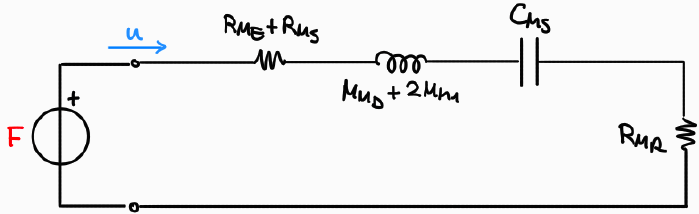
\includegraphics[width=0.60\linewidth]{high_freq_circuit.png}
    \caption{Complete mechanical equivalent circuit for the derivation of the kinematic transfer functions. The voice-coil driving force \(F = Bl i_c\) excites the series combination of the total mechanical resistance \(R_M\), the moving mass \(M_{MS}\), and the suspension compliance \(C_{MS}\)}
    \label{fig:highFreqCircuit}
\end{figure}

\subsection{Voice-Coil Velocity}
\label{ssc:731}

Starting from the driving force \(F_\mathrm{RMS} = Bl v_g/(R_g + R_{EC})\) and the total mechanical impedance \(Z_M\), the voice-coil velocity is:
\[
u_C = \frac{F}{Z_M} = \frac{v_g}{Bl} \frac{1}{Q_{ES}} \beta_C(f)
\]
where the normalized velocity transfer function is:
\begin{equation}
    \beta_C(f) = \frac{j\dfrac{f}{f_s}}{1 - \left(\dfrac{f}{f_s}\right)^2 + j\dfrac{1}{Q_{TS}}\dfrac{f}{f_s}}
    \label{eq:betaC}
\end{equation}
The magnitude \(|\beta_C|\) peaks at \(f = f_s\) with value \(Q_{TS}\), rising as \(f/f_s\) below resonance and falling as \(f_s/f\) above it.

\begin{figure}[!htb]
    \centering
    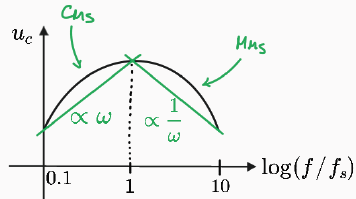
\includegraphics[width=0.60\linewidth]{u_c(f).png}
    \caption{Normalized voice-coil velocity \(|u_C|\) as a function of \(\log(f/f_s)\). The velocity rises as \(f\) in the stiffness-controlled region, peaks at resonance, then decays as \(1/f\) in the mass-controlled region above \(f_s\)}
\end{figure}

\subsection{Diaphragm Displacement}
\label{ssc:732}

Displacement is the time integral of velocity, so in the sinusoidal regime \(x_C = u_C/(j\omega)\):
\[
x_C = \frac{v_g}{Bl} \frac{1}{Q_{ES}} \frac{1}{2\pi f_s} \gamma_C(f)
\]
where the normalized displacement transfer function is:
\begin{equation}
    \gamma_C(f) = \frac{1}{1 - \left(\dfrac{f}{f_s}\right)^2 + j\dfrac{1}{Q_{TS}}\dfrac{f}{f_s}}
    \label{eq:gammaC}
\end{equation}
Below resonance, where the compliance dominates, \(\gamma_C \approx 1\) and the displacement is constant, equal to \(F C_{MS}\): the cone moves like a spring-loaded body with excursion set entirely by the suspension stiffness.
This is the stiffness-controlled regime.

\begin{figure}[!htb]
    \centering
    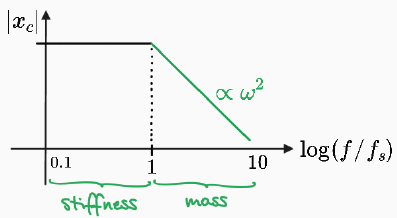
\includegraphics[width=0.60\linewidth]{x_c(f).png}
    \caption{Normalized diaphragm displacement \(|x_C|\) as a function of \(\log(f/f_s)\). Below \(f_s\) the displacement is constant (stiffness-controlled); at resonance it peaks by a factor \(Q_{TS}\); above \(f_s\) it falls as \(1/f^2\) in the mass-controlled region}
\end{figure}

\subsection{Diaphragm Acceleration and the Mass-Controlled Regime}
\label{ssc:733}

Acceleration is the time derivative of velocity, so \(a_C = j\omega u_C\):
\[
a_C = \frac{v_g}{R_g + R_{EC}} \frac{Bl}{M_{MS}} \alpha_C(f)
\]
where the normalized acceleration transfer function is:
\begin{equation}
    \alpha_C(f) = \frac{-\left(\dfrac{f}{f_s}\right)^2}{1 - \left(\dfrac{f}{f_s}\right)^2 + j\dfrac{1}{Q_{TS}}\dfrac{f}{f_s}}
    \label{eq:alphaC}
\end{equation}

\begin{figure}[!htb]
    \centering
    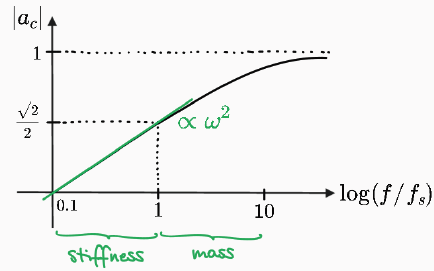
\includegraphics[width=0.60\linewidth]{a_c(f).png}
    \caption{Normalized diaphragm acceleration \(|a_C|\) as a function of \(\log(f/f_s)\). The acceleration rises as \(f^2\) below resonance, peaks at \(f_s\), then becomes constant in the mass-controlled region above \(f_s\). Since far-field pressure is proportional to acceleration, this plateau corresponds to a flat acoustic pressure response}
\end{figure}

\paragraph{The mass-controlled plateau} Above resonance, where \(f \gg f_s\), the inertial term \(\omega M_{MS}\) dominates the mechanical impedance and \(\alpha_C(f) \to -1\), so:
\[
a_C \approx \frac{v_g}{R_g + R_{EC}} \frac{Bl}{M_{MS}} = \text{const}
\]
The acceleration is independent of frequency, depending only on the ratio \(Bl/M_{MS}\) and the source voltage.
Correspondingly, the velocity decays as \(u_C \propto 1/f\) and the displacement falls as \(x_C \propto 1/f^2\), so cone excursion at high frequencies is naturally suppressed.
The far-field acoustic pressure, being proportional to diaphragm acceleration, is therefore flat above \(f_s\): this is the design target for a broadband loudspeaker, and it explains why the mass-controlled region is the primary operating band of a woofer.
